%!TEX root = ../deco_star.tex


%-------------------------------------------------------------------------
%-------------------------------------------------------------------------
\section{Taxonomy of Control Mechanisms}
\label{sec:taxo_control_mechanism}


% % WHY IS THIS A DIFFICULT PROBLEM

% To offer creative means is a layered process. At its core, the generating algorithm should ease the creation process for an artist and fully use the benefits of computational control. However, the algorithm also has to be flexible enough to allow for various interaction methods and individual design goals. There is a delicate balance between giving artists as much control as is needed without burdening them with unwanted details and tedious manufacturing. Similarly, this analysis framework is multi-layered to distill and summarize the different aspects of creative control.
% % WHAT DID THE OTHER RELATED TO THE PROBLEM?

% % WHAT ARE WE GOING TO DO ABOUT IT?

A discussion of creative means cannot be derived directly from the related work. Past authors have followed various motivations and have emphasized different aspects when describing their work and results. In order to classify the work in an objective and unified manner, we analyze the actual presented control mechanisms and relate them to general control paradigms. Based on this analysis, we then can also investigate the creative means. While the classification of the control mechanisms can be directly taken from the authors' descriptions (\Cref{sec:analysis}~\nameref{sec:analysis}), its following discussion of the creative means has an interpretative nature to it. 

We now lay the groundwork for our later evaluation of control mechanisms of the state of the art. As guide for our review of references, we first dissect a creation process into overall control paradigms and classify specific control mechanisms by their interaction types. The following taxonomy shows the capabilities of the different control mechanisms and potential trade-offs between approaches.  

\newcommand{\controlParamsFigWidth}{1.0}

\subsection{Control Paradigms}

A creation process can be described by answering the questions of \textit{how}, \textit{what}, \textit{where}, \textit{when} and \textit{who}. These paradigms can be discussed in various creation contexts and could even be translated to traditional media such as aquarell on paper.

\subsubsection{How}

How is a control executed or an input given by an artist? How far is it from the visual result on the canvas?


\textit{File}: The control is externally given, such as with code or a configuration file.

\textit{UI}: A separate UI is given through which an artist gives input and activates states. User interfaces are often in close proximity to the canvas, carefully designed and easily usable. However, because they detach the work from the actual output, UIs still have an abstract nature. An artist must actively translate his or her interaction with the UI to the resulting output on the canvas.

\textit{On canvas}: Controls are executed directly on the output canvas. Most of these controls require an activation or selection of a tool in a separate UI, such as selecting a pen for drawing on a canvas. In this case we consider the pen primarily as a control mechanism. There are cases where controls cannot clearly be classified as either UI or on canvas. A pen, for example, can have different characteristics that an artist needs to set in the UI. Ideally, the adjustment of settings should be as seamlessly integrated into an on-canvas tool as possible (e.g., with selection choices appearing as tool tips).

\begin{figure}[H]
    \centering
        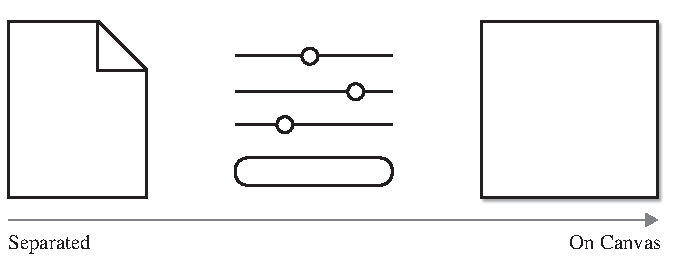
\includegraphics[width=\controlParamsFigWidth\linewidth]{figures/control_paradigms/how.pdf}
\end{figure}


\subsubsection{What}

What does an artist give as input? What is the level of abstraction of the content that an artist works with?

\textit{Code}: Input is a syntactically structured and formal language.

\textit{Value}: The input is a single value, chosen from a range - for example, with a slider.

\textit{Intermediate}: The input is visual but still of an abstract nature, such as controlling sketches for a mask or arrows for directionality. Again, artists have to interpret how these inputs affect the result.

\textit{Element}: The input constitutes a component of the resulting pattern.

\begin{figure}[H]
    \centering
        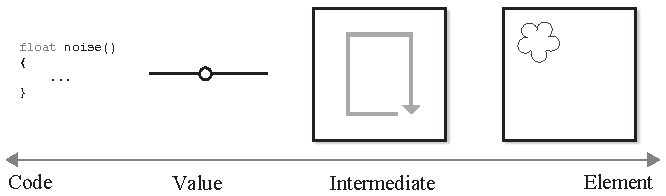
\includegraphics[width=\controlParamsFigWidth\linewidth]{figures/control_paradigms/what.pdf}
\end{figure}



\subsubsection{Where}

Where does the input have an effect spatially and what is its area of influence?

\textit{Global}: The input has global influence (e.g., by filling the whole space or by adjusting all elements on the canvas).

\textit{Region}: The input has an effect in a region of the canvas (e.g., on a drawn curve).

\textit{Local}: The input has an effect on one specific element.

\begin{figure}[H]
    \centering
        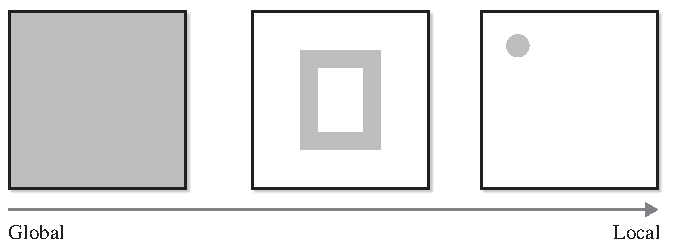
\includegraphics[width=\controlParamsFigWidth\linewidth]{figures/control_paradigms/where.pdf}
\end{figure}


\subsubsection{When}

When can input be given and at what time in the creation process is the control executed?

\textit{Before}: Input is given before the actual creation process.

\textit{During}: Input is given during the creation process, when parts of the results are already visible. This is typically a painting mechanism. However, some processes can also be paused and adjusted.

\textit{After}: Input is given after the creation process. The result is visible to the artist and can be adjusted retrospectively.

\begin{figure}[H]
    \centering
        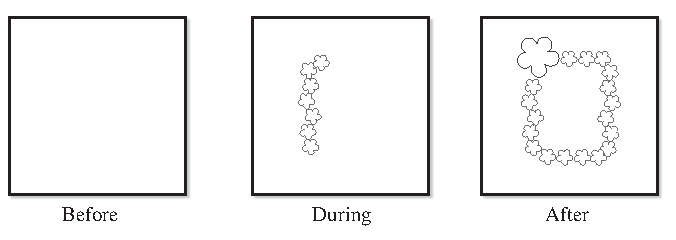
\includegraphics[width=\controlParamsFigWidth\linewidth]{figures/control_paradigms/when.pdf}
\end{figure}


\subsubsection{Who}

Who can give the input in regard to the type of skill set needed? This category can be in part derived from the above characteristics of \textit{how} and \textit{what}. In most general terms this category can be classified as the following.


\textit{Programmer}: To give input with dissecting analytical-formal and logical thinking and the ability to abstract.

\textit{Artist}: To give input with comprehensive intuitive-visual and spatial thinking and the ability to create (e.g., by drawing).

\begin{figure}[H]
    \centering
        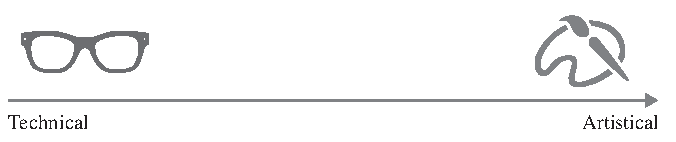
\includegraphics[width=\controlParamsFigWidth\linewidth]{figures/control_paradigms/who.pdf}
\end{figure}

The who category is listed here for completeness. However, to fully answer the questions of needed competencies, skill- and mindsets, including the accompanying psychological and artistic aspects, is out of the scope of this thesis and requires knowledge in fields other than computer science. The following discussions are rooted in computer graphics research and aim for an assessment of algorithmic controllability. Hence, the classification of who specifically is most suitable to use a tool, is put aside.


\subsection{Control Mechanisms}
\label{subsec:taxo_control_mechanism}

For a meaningful analysis, the above classification must be further broken down into the specific control mechanisms. 
% These are described for each technique by the authors of that publication. 
% For the assessment of a mechanism, the \textit{how}, \textit{what}, \textit{where} and \textit{when} are interdependent, as Table~\ref{table:taxo_controlmechanism} indicates and what is further discussed in .

The following low-level characteristics categorize input modes and their primary effect. Because this survey focuses on interfacing algorithms, UI specifics, such as the layout of buttons, are not considered. Once the specific control mechanisms are analyzed, they constitute a method in combination with the above control paradigms.

\subsubsection{Initialization}



\textit{System Configuration}: Required overall setup of the system, such as computing caches or training a model. This is usually a one-time investment.

\textit{Task Initialization}: A non-creative task that has to be executed each time in order to produce an output, such as selecting the specific optimization algorithm.



\subsubsection{Exemplars}


\textit{Image}: An example image that should be matched in its entirety. Examples are usually pixel data.

\textit{Element Arrangement}: An example element arrangement that should be matched in its entirety. Elements are usually separate shapes and might carry additional data.

\textit{Element}: One specific asset that becomes in the result part of a whole. Elements can be shapes or pixel data.


\subsubsection{Parameterization}


\textit{Visual Output}: Parameters that can adjust visual features directly in the output.

\textit{System/Generation}: Parameters that influence the output indirectly, such as parameters for an optimization algorithm or constraints.


\subsubsection{Handling}


\textit{Visualization}: Any type of visual interface that goes beyond the standard UI elements, such as sliders and buttons.

\textit{Image-Based}: Images as indirect control input, such as pixel data masks.

\textit{Sketch-Based}: Sketches and curves directly put on the canvas - for example, the drawing of a mask with a pen tool.


\subsubsection{Filling}


\textit{Shapes}: A space to fill (e.g., a specific shape).

\textit{Masking}: Areas within the shape to fill that should remain unaffected.

\textit{Curves to Fill}: A one-dimensional curve or path to be filled. The curve is given as a whole before the filling starts.


\subsubsection{Guiding}


\textit{Painting/Strokes to Follow}: A curve, usually created by mouse movements or with a stylus pen, that is filled with output elements while the curve is generated - often understood as brushing.

\textit{Directions}: Visual elements such as intermediate curves, arrows or output components that define directions for the design to follow (e.g., with an underlying vector field).


\subsubsection{Placing}


\textit{Element Placement}: The direct placement of components on the canvas as part of the final result.

\textit{Element Drag \& Drop}: Drag and drop of components on the canvas within the existing result.


\subsubsection{Control Stages of the Mechanisms}
\label{subsec:taxo_control_mechanism}

\subimport{tables/}{table_controlmechanism}
% \subimport{tables/}{table_vectorfield}

For interrelating the control mechanisms to the control paradigms, we considered the publications that are investigated in \cref{sec:analysis}~\nameref{sec:analysis}. Due to the diversity of the underlying methods and the different design goals of the considered body of work, we believe this to be a representative summarization.

\majortodo[inline]{Update Table.}

Table~\ref{table:taxo_controlmechanism} shows that global, hence automatic, control is usually enabled through intermediate representations, such as an example image, while on the other end of the spectrum, the placement of elements as part of the actual output is local, and automation is lost.

Parameterization and the different types of handling also require abstracted input from an artist, such as the use of a slider. Sketch-based controls, such as an eraser, move the interaction onto the canvas and can make small-scale adjustments. The definition of a space or a curve to fill and masking areas is also usually done directly on the canvas but only influence the output indirectly.

A painting mechanism simultaneously creates the output directly on the canvas but can only do so in a limited region depending on the brush size. All other inputs are typically given before or after the generation of the output.

This classification underlines that a focus on one control type, as is usual in computer graphics research, leads to the common trade-off between global automation and local manual manufacturing. In order to support creative work, control mechanisms need to be combined in a novel and unified manner.

